\addcontentsline{toc}{chapter}{Appendices}
\appendix

\chapter{Eigenvalue Distributions of Derivative Operators}
\label{appendix:eigenvalue-distributions}
Using the Circular Diagonalization Theorem \cite{Ingleton1956TheMatrices} one can derive the eigenvalues $\lambda_k$ of an $K\times K$ matrix which represents the second-order central difference approximation to the second derivative on $K$ sites of a one dimensional ring
\begin{align}
	\frac{\partial^2}{\partial x^2} \rightarrow
	\begin{pmatrix}
	  -2 & 1 &  &  &  & 1 \\
	  1 & -2 & 1 &  &  &  \\
	  & 1 & \ddots & \ddots &  & \\
	  & & \ddots & \ddots & 1 & \\
	  & & & 1 & -2 & 1 \\
	  1 & & & & 1 & -2 \\
	\end{pmatrix}\\
	\begin{matrix}
	  \lambda_k =2\left(\cos\left(\frac{2\pi k}{K}\right)-1\right) \\
	  k\in\{0,1,\cdots,K-1\}
	\end{matrix}
	\qquad
\end{align}
As the number of sites $K\rightarrow\infty$ the argument $k/K\in[0,1]$
and the eigenvalues remain bounded $-4<\lambda_k<0$. By shifting and scaling
the index $k\rightarrow\frac{k-K\pi}{2\pi}$ the eigenvalues are expressed as
a dispersion relation
\begin{align}
  \lambda(k)&=
  -2\left(\cos k+1\right)
  \quad k\in[-\pi,\pi]
\end{align}
The discrete $L$-dimensional Laplacian is simply the Kronecker sum $\oplus$ of one
dimensional cases and thus its eigenvalues are simply the sum over one dimensional dispersions \cite{Laub2004MatrixEngineers}
\begin{align}
  \lambda(k)&=
  -2\sum_{i=1}^L\left(\cos k_i+1\right)
  \quad k\in[-\pi,\pi]^L
\end{align}
The probability density $P(\lambda)$ can be expressed as a density integral
over the $L$-dimensional hypercube region $[-\pi,\pi]^L$
\begin{align}
	P(\lambda')&=\frac{1}{Z}\int_{[-\pi,\pi]^L}\!\delta(\lambda'-\lambda(k))\,\mathrm{d}k
\end{align}
We proceed with an element-wise change of variables $u=2\cos k$ and recognise that the integration region is $L$-fold symmetric across each component axis, which allows restriction of the domain of integration to a hyper-octant. In coordinates $u$ the region becomes $[-2,2]^L$
\begin{align*}
  P(\lambda)&=\frac{1}{Z}
  \int_{\Omega'}\!
  \frac{\delta(\Lambda_L+\sum_{i}u_i)}
  {\sqrt{\prod_{i=1}^L(1-u_i^2/4) }}
  \,\mathrm{d}u
  \qquad
  \begin{matrix}
    \Lambda_L=\lambda+2L \\
    |\Lambda_L|\leq2L
  \end{matrix}\\
  &=\frac{1}{2\pi Z}
  \int_{-\infty}^{\infty}\int_{\Omega'}\!
  \frac{\mathbb{e}^{\Lambda_L Ik}\exp[\sum_{i}u_i Ik]}
  {\sqrt{\prod_{i=1}^L(1-u_i^2/4) }}
  \,\mathrm{d}u\mathrm{d}k\\
  &=\frac{1}{2\pi Z}
  \int_{-\infty}^{\infty}\mathbb{e}^{\Lambda_L Ik}
  \prod_{i=1}^L\int_{-2}^{2}\!
  \frac{\mathbb{e}^{u_i Ik}}
  {\sqrt{1-u_i^2/4}}
  \,\mathrm{d}u_i\mathrm{d}k
\end{align*}
The Fourier representation of the delta function allowed the
factorisation of the integral. We recognise a repeated Bessel integral and replace it with the Bessel function of the first kind $J_n(k)$, leaving only a Fourier transform which we define as $\mathcal{F} : f\rightarrow \frac{1}{\sqrt{2\pi}} \int_{-\infty}^{\infty}f(k)e^{ I\Lambda k}\mathrm{d}k$
where
\begin{equation*}
    f(k) = \frac{1}{\sqrt{2\pi}Z}\prod_{i=1}^L\int_{-2}^{2}\!
  \frac{\mathbb{e}^{u_i Ik}}
  {\sqrt{1-u_i^2/4}} \mathrm{d}u_i
\end{equation*}
To clean the formula up even further we may use the convolution theorem to deal with the powers of $L$, leaving only the Fourier transform of the Bessel function $J_0(k)$, which is the arcsine distribution $\alpha(\lambda)$. The eigenvalue density of a Kronecker sum of matrices is the convolution of the densities of those matrices.
\begin{align}
  P(\lambda)=\underbrace{
  \alpha(\lambda)*\alpha(\lambda)*\cdots*\alpha(\lambda)}_{L}\qquad\qquad\label{eq:mlap}\\
    \alpha(\lambda)=
      \frac{\Pi\left(\frac{\lambda+2}{2}\right)}{2\pi\sqrt{1-\left(\frac{\lambda+2}{2}\right)^2}}
    \qquad
    \Pi(x)=
      \begin{cases}
        1 & |x|<1\\
        0 & |x|\geq1\\
      \end{cases}
	\label{eq:laplacian-distribution}
\end{align}
\begin{Figure}
    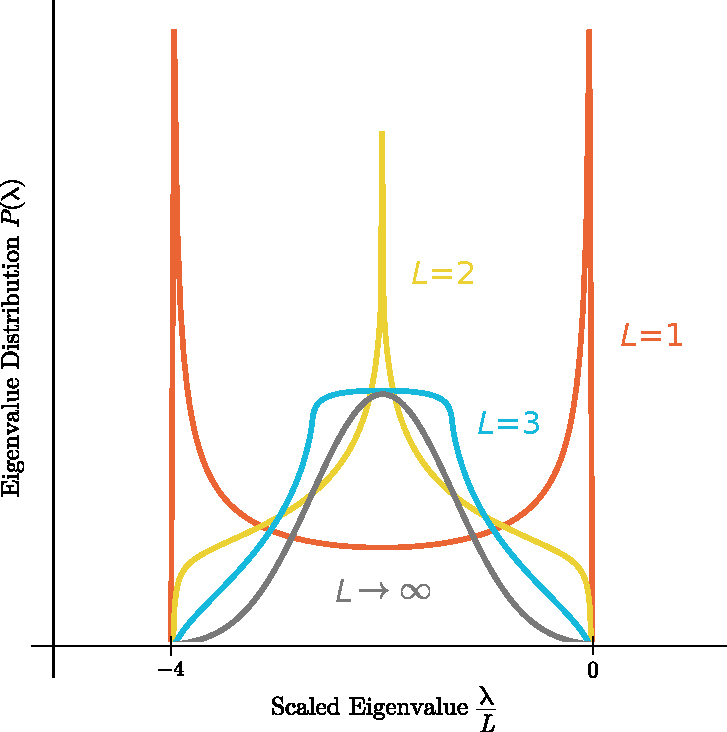
\includegraphics[width=0.6\linewidth]{laplacian-spectra}
    \caption{Eigenvalue distributions $P(\lambda)$ of the $L$-dimensional Laplacian}
    \label{fig:laplacian-spectra}
\end{Figure}
The one dimensional density has two Van Hove singularities at $\lambda=-4,0$ given by the arcsine law $\alpha(\lambda)$, whereas the two dimensional case has one at $\lambda=-4$ given by the complete elliptic integral of the first kind $K(m)$. Figure \ref{fig:laplacian-spectra} reveals that in higher dimensions singularities do not occur; instead there appear to be discontinuities in the higher order derivatives. The density smooths out as repeated convolutions bring it to a normal distribution; this is another way to state the Central Limit Theorem. In the context of diffusion, the Laplacian is scaled by the diagonal diffusion matrix. To take this scaling into account, components $D_i$ are introduced in the arcsine laws
\begin{align}
	\alpha(\lambda) \rightarrow \frac{1}{D_i}\alpha(\lambda/D_i)
\end{align}
The eigenvalue distributions determine the eigenbasis evolution  \eqref{eq:eigenbasis-vector-evolution} which reveals that the second order derivative leads to exponential relaxation of all basis vectors, except for the subset with vanishing eigenvalue $\lambda=0$. The corresponding zero eigenvectors $v_0$ are the Fourier components of the steady state distribution, and are the only components that remain as $t\rightarrow\infty$. The diffusive components $D_i$ determine the timescale of relaxation in each dimension.


\chapter{Interpretation of Morphogen Gradients by a Bistable Circuit}
\label{appendix:double-exclusive}
\includepdf[pages=1-51, offset=75 -90, scale=0.85, frame,
        clip,trim=20mm 5mm 20mm 15mm,
        pagecommand={}, addtotoc={
                2,section,1,Supplementary Figures,appendix:double-exclusive:figures,
                18,section,1,Supplementary Methods,appendix:double-exclusive:methods,
                19,subsection,2,Differential Equation Models \& Parameter Inference,appendix:double-exclusive:inference,
                40,subsection,2,Bistability Analysis,appendix:double-exclusive:bistability,
                42,subsection,2,Boundary Experiments,appendix:double-exclusive:boundaries,
                50,subsection,2,Models of the Exclusive Receiver Relay Circuits,appendix:double-exclusive:relay},
        addtolist={
                2, figure, {\textit{Supplementary Figure 1}\quad Circuit variants}, fig:double-exclusive:variants,
                4, figure, {\textit{Supplementary Figure 2}\quad Raw timecourse fluorescence traces}, fig:double-exclusive:plate-data,
                15, figure, {\textit{Supplementary Figure 13}\quad Hysteresis flow cytometry experiments}, fig:double-exclusive:flow-hysteresis,
                41, figure, {\textit{Supplementary Figure 25}\quad Bifurcation curves for uniform and protected degradation models}, fig:double-exclusive:degradation-models,
                41, figure, {\textit{Supplementary Figure 26}\quad Bifurcation curve insensitivity specific growth rate $\gamma_0$}, fig:double-exclusive:growth-rate-sensitivity
}]{publications/double-exclusive-si.pdf}

\chapter{Parameter Inference with Bifurcation Diagrams}
\label{appendix:inference}
\includepdf[pages=1-6, offset=75 -90, scale=0.85, frame,
        clip,trim=33mm 20mm 33mm 20mm,
        pagecommand={}, addtotoc={
                1,section,1,Bifurcation Diagrams as Tangent Fields,appendix:tangent-fields,
                2,section,1,Bifurcation Measure Properties,appendix:bifurcation-measure,
                3,section,1,Leibniz Rule for Space Curves,appendix:leibniz-rule,
                5,section,1,Application to the Double Exclusive Model,appendix:more-complex-model,
                6,section,1,Extension for Hopf Bifurcations,appendix:hopf-measure},
        addtolist={
                1, figure, {\textit{Supplementary Figure 1}\quad Two implicit surfaces $f_{\theta}(z)=0$ and $g_{\theta}(z)=0$ in $\mathbb{R}^3$ intersecting to form a space curve which is tangent to field $\tangent(z)$ and perpendicular to gradients $\partial_{z}f_{\theta}$ and $\partial_{z}g_{\theta}$}, fig:implicit-surfaces,
                2, figure, {\textit{Supplementary Figure 2}\quad Left/Right : Determinant $\Det$ and tangent field $\tangent(z)$ for the saddle-node/pitchfork models for some set values of $\theta$ revealing that $\Det=0$ defines bifurcations}, fig:determinant-field,
                5, figure, {\textit{Supplementary Figure 3}\quad Bifurcation inference for the \emph{double exclusive reporter}. A. Optimal parameter estimates $\theta^*$ for the targets $\targets=\{1,2\}$ (indicated by yellow lines in panel B) reveal four regions  with two geometrically different regimes: mutual activation (region 1) and mutual inhibition (regions 2-4). B. Example bifurcation diagrams indicate that region 2 has swapped kinetics between $L$ and $T$ to region 3. Region 4 has models with non-zero imaginary parts to eigenvalues indicating damped oscillations (shown in light green).},
                fig:double-exclusive-optima,
                6, figure, {\textit{Supplementary Figure 4}\quad Bifurcation measure $\measure(s)$ and eigenvalues $\lambda(s)$ along the arclength $s$ for two different bifurcation curves demonstrating how the measure detects non-zero imaginary parts $\Imag[\lambda]$ (onset of damped oscillations marked by circle) and sign changes in real parts $\Real[\lambda]$ (Hopf bifurcations marked by stars)},
                fig:hopf-measure
}]{publications/bifurcation-inference-si.pdf}

\chapter{Exploring Bifurcations between Phenotypes}
\label{appendix:exploring}

\section{Experimental Methods}
\subsection{Tissue Acquisition \& Dissociation} 

All samples were collected via the \href{https://www.cbtm.group.cam.ac.uk}{Cambridge Biorepository for Translational Medicine} under Research Ethics Committee approval 15/EE/0152. Tissue was obtained from five deceased organ donors following circulatory death. Donor metadata is given in Table \ref{table:donors}. Briefly, following cessation of circulatory function donors proceeded to organ donation. Organs were perfused \emph{in situ} with cold organ preservation solution and cooled with topical application of ice. Samples for the study were obtained within 60 minutes of cessation of circulation and placed in University of Wisconsin organ preservation solution for transport at 4°C to the laboratory. Lung and liver samples were obtained from the left lower lobe of the lung and the right lobe of the liver. In addition, two donor-matched blood samples were collected prior to withdrawal of life support, under approval 97/290.

To minimise the possibility of processing-depended differences in cell surface marker expression, all samples, including blood, were processed using enzymatic digestion protocol. Briefly, solid tissues were weighed, transferred into 10cm tissue culture dishes and cut into small pieces. Up to 5g of tissue was then transferred to each of eight GentleMACS C tubes (Miltenyi Biotec) containing 5mL of dissociation media composed of X-vivo15 supplemented with 0.13U/mL Liberase TL (Roche), 10U/mL Benzonase nuclease (Millipore/Merck), 2\% (v/v) heat-inactivated fetal bovine serum (FBS, Gibco), penicillin (100 U/ml, Sigma-Aldrich), streptomycin (0.1 mg/ml, Sigma-Aldrich), and 10mM HEPES (Sigma Aldrich). The samples were then dissociated on a GentleMACS Octo dissociator (Miltenyi Biotec) running a protocol that provided gradual ramping up of homogenisation speed and two 15 minute heating/mixing steps at 37°C. Digested tissue was passed through a 70$\mu$m MACS Smartstrainer (Miltenyi Biotec) and the flow-through was first washed with media supplemented with 2 mM EDTA and then with PBS. Mononuclear cells were enriched by Ficoll-Paque (GE Healthcare) density centrifugation according to manufacturer's instructions. Following, density centrifugation, mononuclear layer was collected, washed once with PBS and cell pellet was resuspended in FACS buffer (PBS, 2.5$\%$ FBS).

Bone marrow aspirates and peripheral blood samples were first subjected to Ficoll-Paque density centrifugation, according to manufacturer's instructions, the mononuclear layer was then collected, washed with PBS and cells were treated with the same dissociation media as solid tissues for 30 min at 37°C prior to washing and resuspension in FACS buffer.

\subsection{Flow Cytometry}

Depending on the cell yield, up to 1x10\textsuperscript{6} mononuclear cells/tissue were stained with antibodies shown in Table \ref{table:panel}. Not all donors were stained with the same panel. To expand total number of markers, sentinel panel design was implemented where CD3 and IgD were detected with antibodies conjugated to BUV395 and Foxp3 and IgM were detected with antibodies conjugated to PE in some donors. Refer to Table \ref{table:panels} for details. 

Single cell suspensions were washed once in PBS, transferred into 96 v-bottom plate and stained with Zombie UV viability dye for 30 min at 4°C following by a wash with FACS buffer. Cell pellets were resuspended in 50$\mu$l FACS buffer with Human FcR block (BD Biosciences) and incubated for 10 min at 4°C. Next, cells were pelleted, excess buffer removed and 100$\mu$l of antibody master mix composed of cell-surface antibody cocktail (see Table \ref{table:panels}), BV buffer (BD) and True-Stain Monocyte Blocker (Biolegend) and incubated for 1h at 4°C. Following incubation, cells were washed three times in PBS and prepared for intracellular staining using transcription factor fixation/permeabilisation kit (eBioscience) according to the manufacturer's instructions. Following IC staining, cell were resuspended in PBS and analysed on BD FACSymphony A3 cell analyser within 10 hours.

\section{Supplementary Tables}

\begin{landscape}
\begin{table}
\footnotesize
\begin{center}
\begin{tabular}{>{\centering\arraybackslash}p{0.6cm}>{\centering\arraybackslash}p{0.4cm}>{\centering\arraybackslash}p{0.7cm}>{\centering\arraybackslash}p{0.9cm}>{\centering\arraybackslash}p{0.9cm}>{\centering\arraybackslash}p{0.9cm}>{\centering\arraybackslash}p{1cm}>{\centering\arraybackslash}p{1cm}>{\centering\arraybackslash}p{1cm}>{\centering\arraybackslash}p{1cm}>{\centering\arraybackslash}p{2.1cm}>{\centering\arraybackslash}p{0.6cm}}
    \toprule
    Donor ID & Sex & Age & Primary cause of death & Multi-trauma & Days in hospital & BMI &CMV/ EBV/ TOXO& Smoking & Alcohol (u/day) & Antibiotics within 2 weeks of death & Steroids \\
    \midrule
    390C & F & 65-70 & ICH & \cmark & 2 & 30-35 & $+$/$+$/$-$ & ? & $<$1 & \xmark & \xmark \\
    403C & M & 50-55 & ICH & \cmark & 8 & 30-35 & $+$/$+$/$-$ & \cmark & $<$1 & Co, T & \xmark \\
    423C & M & 60-65 & ICH & \xmark & 2 & 20-25 & $-$/$+$/$-$ & \cmark & $>$9 & G, F & D \\
    412C & M & 70-75 & ICH & \xmark & 5 & 26-30 & $-$/$+$/$+$ & \cmark & $<$2 & A$^\star$ , F, G, C, Co & P$^\dagger$ \\
    428C & F  & 55-60 & ICH & \xmark & 3 & 20-25 & $-$/$+$/$-$ & \cmark & $>$9 & Co & \xmark \\
    \bottomrule
\multicolumn{12}{p{\linewidth}}{\vline height10pt width0pt
\relax F = Female; M = Male; ICH = intracranial haemorrhage; CMV = Cytomegalovirus; EBV = Epstein-Barr virus; TOXO = Toxoplasmosis; Co = Co-amoxiclav; A = Amoxicillin; T = Tazocin; F = Flucloxacillin; G = Gentamicin; D = Dexamethasone; C = Clarithromycin; \cmark = Yes; \xmark = No; ? = Not known;P = Prednisolone; $^\star$pre-admission, $^\dagger$pre-treatment}\\
\end{tabular}
\caption{Donor Metadata}
\label{table:donors}
\end{center}
\end{table}
\end{landscape}

\begin{table}
\footnotesize
\begin{center}
    \begin{tabular}{llll}
        \toprule
        Specificity & Fluorochrome & Clone & Source \\
        \midrule
        CD3 &  BUV395 & SK7 & BD \\
        CD8 & BUV563 & RPA-T8 & BD \\
        CD69 & BUV737 & FN50 & BD \\
        CD4 & BUV805 & SK3 & BD \\
        CD4 & BUV661 & SK3 & BD \\
        CD45 & BUV805 & HI30 & BD \\
        CD103 & BV421 & Ber-ACT8 & BD \\
        HLA-DR & BV510 & G46-6 & BD \\
        CD127 & PE-Cy7 & HIL-7R-M21 & BD \\
        CCR4 & BV605 & L291H4 & Biolegend \\
        CCR6 & BV650 & 11A9 & BD \\
        PD-1 & BV711 & EH12.1 & BD \\
        CD45RA & BV786 & HI100 & BD \\
        CCR10 & BB515 & 1B5 & BD \\
        CXCR3 & BB700 & 1C6/CXCR3 & BD \\
        CXCR5 & APC-R700 & RF8B2 & BD \\
        CCR7 & APC-Fire750 & G043H7 & Biolegend \\
        CD25 & APC & M-A251 & BD \\
        CD25 & APC & 2A3 & BD \\
        CD19 & BV570 & HIB19 & Biolegend \\
        IgM & PE & G20-127 & BD \\
        IgD & BUV395 & IA6-2 & BD \\
        Foxp3 & PE & 269D/C7 & BD \\
        Foxp3 & PE & PCH101 & eBioscience \\
        Helios & PE-Dazzle & 22F6 & Biolegend \\
        Zombie UV & - & - & Biologend \\
        \bottomrule
    \end{tabular}
\caption{Details of antibodies used in this study}
\label{table:panel}
\end{center}
\end{table}

\begin{table}
\footnotesize
\begin{center}
    \begin{tabular}{lrlll}
        \toprule
        & \multicolumn{4}{c}{Fluorochromes} \\
        \cmidrule{3-5}
         & Panels:&  A &  B &  C \\
        \cmidrule{3-5}
        Specificity & Donor:& 390C & 403C & 412C, 423C, 428C \\
        \midrule
        CD45 && BUV805 & - & - \\
        CD19 && - & - & BV570 \\
        IgM && - & - & PE \\
        IgD && - & - & BUV395 \\
        CD4 && \textbf{BUV661} & \textbf{BV805} & \textbf{BV805} \\
        CD3 &&  BUV395 & BUV395 & BUV395 \\
        CD8 && BUV563 & BUV563 & BUV563 \\
        CD69 && BUV737 & BUV737 & BUV737 \\
        CD103 && BV421 & BV421 & BV421 \\
        HLA-DR && BV510 & BV510 & BV510 \\
        CD127 && PE-Cy7 & PE-Cy7 & PE-Cy7 \\
        CCR4 && BV605 & BV605 & BV605 \\
        CCR6 && BV650 & BV650 & BV650 \\
        PD-1 && BV711 & BV711 & BV711 \\
        CD45RA && BV786 & BV786 & BV786 \\
        CCR10 && BB515 & BB515 & BB515 \\
        CXCR3 && BB700 & BB700 & BB700 \\
        CXCR5 && APC-R700 & APC-R700 & APC-R700 \\
        CCR7 && APC-Fire750 & APC-Fire750 & APC-Fire750 \\
        CD25 && APC & APC & APC \\
        Foxp3 && PE & PE & PE \\
        Helios && PE-Dazzle & PE-Dazzle & PE-Dazzle \\
        Zombie UV && Zombie UV & Zombie UV & Zombie UV \\
        \bottomrule
    \end{tabular}
\caption{Immunophenotyping panel designs used in the dataset}
\label{table:panels}
\end{center}
\end{table}